\section{Design and Implementation}

Altough some projects build entire or partially custom blockchain network software, using a framework like Hyperledger Composer is a much more streamlined way to get a fast functioning prototype.

The baseline for the design will be the written list of requirements, mainly the functional requirements part, and the specifications of the Hyperledger projects.

The design can be divided into 4 parts:
\begin{itemize}
    \item Model Design for a Composer Business Network
    \item Access Control Design and Identity Management
    \item Network Topology and Deployment
    \item Integrating Existing Systems and Building External Applications
\end{itemize}

These parts are not necessarily sequential, but following the listed order may bring about the best results in development. Since time was an issue and the dissertation already included aspects other than the development, the scope of the development itself could not be broad enough to include a deep exploration of all the aspects listed.

Therefore, the project here presented focuses more on the quality and functional aspects of applying blockchain to the supply chain, and not so much on the quantitative part, which would include tests to the efficiency of the network (throughput, latency). What this means is that the development had a bigger focus on the model design, access control design,identity management and the implementation and validation of these aspects than on building and testing a realistic node topology. The scope for the last item, integrating existing systems and building external applications,was also narrowed down to the essential.

This section is divided in several parts to explain in which way these items were approached, so that conclusions can then be taken to reach an answer to the question: \textbf{"Is it possible to build a feasible architectural design, by using such a tool implement all these requirements?"}
%TODO - places with the thesis questions, they need to be consistent with the use of bold or italic

%Business network definition here, or in the background and mention it here

%Explain that a deployed business network is a ledger that works for a group of companies that wants to form a blockchain for their own supply chain; the network is only as global or as specific as they want it. 

%The designed network here is intended to work for any number of companies

\subsection{Composer Business Network - Model Design}

From the requirements, the business network model for Hyperledger Composer was designed and built. This includes the specifications for the \textit{.cto} file, with the definitions of all class types participants, assets, transactions and events, as well as the enums and concepts (which are basically non-instantiable data types). The script file with the implementation of the transactional code and a query file with custom queries for the blockchain are also explained.

Only the most important data attributes for the classes will be explained, even though \textbf{all of the data attributes from all the classes can be seen on the class diagram exhibited in the annexes.}

\subsubsection*{Participants}

The first step towards designing the system was to define who the users are, in order to model the participants. This is an easy task, as the actors of the system were already defined beforehand.

%PARTICIPANTS
The logical separation for the participant type:
\begin{itemize}
    \item auditor - the participant type that will represent the auditor role; the reason a specific participant type is needed for this actor is so that the access control for the auditors can later be specified;
    \item supplyChainMember - the main participant of the network, the supply chain members are the actual users that will be interacting with each other, so it makes sense that they are modeled; Sub-types were also designed, having in mind that they may exhibit different behaviours, and different access rules can be written based on the sub-type;
    \begin{itemize}
        \item Supplier 
        \item Manufacturer 
        \item Distributor 
        \item Retailer 
        \item Customer
    \end{itemize}
\end{itemize}

Both the auditor and the supply chain member participant types have as attributes some company and personal identification, and the supply chain members also have an account balance, which is the basis for financial transactions.  The reason the admin does not appear here is that the admin of a business network does not need a user type to be able to invoke transactions. Instead, they only need their admin identity card, which in no way needs to be tied to a network participant.

\subsubsection*{Assets}% Concepts and Enums}

Another integral component of the system are the assets, for the asset management aspect of the supply chain. If traceability of products is to be achieved, these products need to be modeled as assets, so that the network can register which ones exist, their status, and any changes that happen.

The proposed assets in this model were: \textbf{Commodity}, \textbf{ShipmentBatch} and \textbf{Contract}. Each of them serves a purpose. A diagram with the assets and their relationships to the participants and each other can be found in Figure \ref{fig:participant_asset}.

\par \textbf{Commodity} - Represents a single product being exchanged, with all its attributes, including the product ID (GTIN), name, description, item status and even the ID of the person who owns it (a participant of the network).
\par \textbf{ShipmentBatch} - Represents a physical shipment, that a buyer orders from a seller. The shipment includes all the tracking information, including tracking number,a shipment status and location. Additionaly, the shipment  has an array of the Commodity items included in it, as well as information on who is the current physical holder of the shipment and owner (other participants). When a shipment is created, since it has an origin and a destination along with other sensible data and shipment conditions, it makes sense that a contract is generated, therefore the shipment also has a contract associated.
\par \textbf{OrderContract} - This represents a digital contract for the conditions of the shipment. The expected arrival location and time, the buyer and seller, as well as a payment price, for when the shipment is delivered (though it is optional). One of the requirements was that contractual agreements should be made possible, as well as financial transactions, and this is the proposed way to make it happen. Fraud checks can also be done on the arrival location, to check if the real arrival location matches the expected one.

\begin{figure}[h]
    \centering
    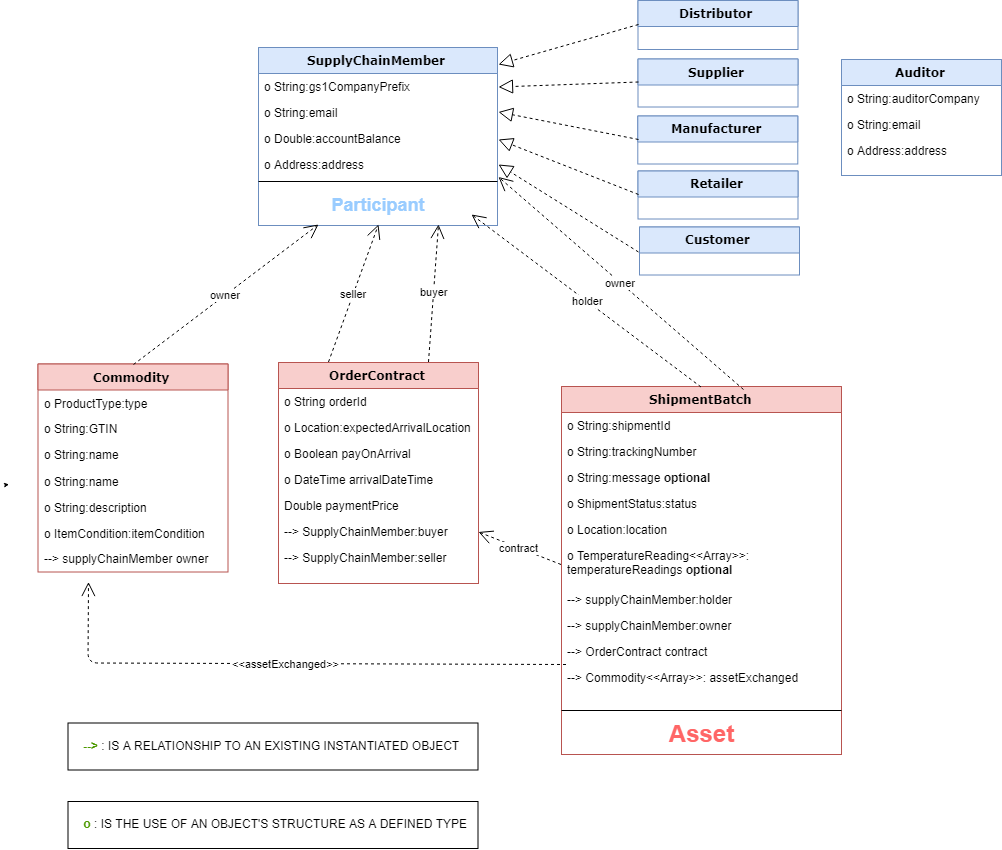
\includegraphics[scale=0.40]{media/participant_asset_relationship.png}
    \caption[Class Diagram for the relationships between assets and participants.]{Class Diagram for the relationships between assets and participants.}
    \label{fig:participant_asset}
\end{figure}

%ASSETS
%CONCEPTS 
%ENUMS

\subsubsection*{Transactions and Transactional Scripts}
The way that the participants an interact with the network and with the assets is through transactions. \textbf{Transactions are the chaincode functions with certain parameters invoked by a user of the network} (how a user can invoke a transaction is another matter, also discussed in the following sections). So, while the participants and assets model the users and data storage of the system, \textbf{the transactions model the behaviour of the network}, by accessing the participant and asset registries and making changes. Any transaction invocation is always recorded in an immutable historical record.

\todo{pedro: por figura nos anexos E e codigo tambem, e referenciar + por algumas cenas em bold}
All the creation, deletion and update transactions are already supported by default by Composer, but all other behaviour needs to be modeled, and sometimes, even these default transactions should be made restricted and replaced by custom made ones, to ensure system integrity.


The transactions that were modeled for this network, with all their parameters can be seen in Figure X, from the annexes, and their code is in Y. What follows is a list of these transactions with their descriptions:
\begin{itemize}
    \item \textbf{CreateShipmentAndContract} - creates a shipment and the associated contract at the same time, for a certain set of parameters, which includes a buyer, seller, the commodities to include in the shipment, etc.
    \item \textbf{UpdateShipment} - update a shipment's tracking status, location and optionally pass it over to a new holder. In case the shipment is being delivered to the buyer, if a payment was established in the contract, it is automatically done. 
    \item \textbf{UpdateCommodity} - A custom transaction to update a commodity, instead of using the default one. The reason is to make access control rules easier for this behaviour easier.
    \item \textbf{DeleteCommodity} - Again, a custom transaction, to delete a commodity. The reason for this transaction being custom is that a verification must be done to check if the commodity is part of a shipment before deleting it. In case it is, to maintain the integrity of the system, the commodity is not deleted
    \item \textbf{ReportDamagedGood} - Sometimes, goods are damaged during their shipment. This transaction updates the current status of a commodity and a description of the occurrence, so that a registry for any damages occurred can be
    \item \textbf{TransformCommodities} - This transaction converts 1 or more commodities in a different set of commodities, by deleting the old ones and creating new ones. It is useful, for instance, when creating a product out of raw materials. 
    \item \textbf{TransferCommodityPossession} - transfer the ownership of a commodity to a different participant of the network, but only if the commodity is not currently part of any shipment.
    \item \textbf{TemperatureReading} - Finally, and to ensure full product condition traceability, temperature readings can be inserted into the system. A shipment can log an array of temperature readings, and each time this transaction is called for a shipment, a reading can be inserted into the array.
\end{itemize}

%\item Tutorial/Show-off the functionalities of some kind? Include this on the 1st point?
\subsubsection*{Queries}
The transactions are used to model actions and behaviour, but to retrieve some of the information, something else is needed, and these are queries. Hyperledger Fabric uses a relational database to store the asset and participant registries and Composer features a way to retrieve the data easily, through filtered queries (using a javascript framework, LoopBack).

\subsection{Composer Business Network - Identity Management and Access Control}

%Identity management - Creating identities, associating them to the participants, etc. (MAYBE THIS IS BETTER OFF IN THE BACKGROUND/STATE OF THE ART SECTION ABOUT COMPOSER)

 % talk about lack of control for multisig? important for when 2 ppl should approve a transaction between them

Permissions - Access control rules:
\begin{itemize}
    \item Transactions
        \begin{itemize}
		\item CreateShipmentAndContract - Anyone (but a customer?) can call this to have a shipment and a contract made;
		\item ReportDamagedGood - Only the holder of a commodity shall be able to submit a damage report for that commodity
		\item TemperatureReading - Only the holder of a commodity shall be able to submit a temperature reading for that commodity (how to do it in case of IoT? -> Prepare the device with the needed business cards)
		\item TransferCommodityPossession - Only the owner of a commodity shall be able to transfer the ownership. This commodity can not be part of a shipment at the moment of the transferrence. 
		\item TransformCommodities - Only the owner of the commodities shall be able to transform them, and he may specify a new owner if he so desires (risky choice, maybe); All transformed commodities in a transaction must have the same owner; (I can comment 1 single line to make this transaction not change owner)
		\item UpdateShipment - Only the holder of a shipment may be able to update its details
		\item UpdateCommodity - Only the owner of a commodity can update it with this transaction
		\item DeleteCommodity - Only the owner of a commodity can delete it
		\end{itemize}
    \item Assets
        \begin{itemize}
        \item Commodity
            \begin{itemize}
			\item Create - Any supply chain member can create commodities, as well as admins; auditors can not;
			\item Read - A supply chain member can only read the commodities it owns or holds; Auditors and admins can read any commodity;
			\item Update - A supply chain member can directly update the commodities it owns; admins can update any commodity;
            \item Delete - Only the admin can delete commodities through this function;
            \end{itemize}
        \item OrderContract
            \begin{itemize}
			\item Create - No one but admin can create
			\item Read - The buyer and the seller can read it; the admin and the auditor can as well
			\item Update - Only the admin can update the contract;
            \item Delete - Only the admin can delete a contract;
            \end{itemize}
        \item ShipmentBatch
            \begin{itemize}
			\item Create - Only the admin can create a shipmentbatch
			\item Read - Only the owner, holder and contract buyer can read the shipment; The admin and auditor can as well;
			\item Update - Only the admin can update the shipment;
            \item Delete - Only the admin can delete the shipment;
            \end{itemize}
        \end{itemize}
    \item Participants
        \begin{itemize}
        \item Supply Members
            \begin{itemize}
			\item No one but admin has permissions to Create, delete or update
            \item Auditor can read any participant; participants can read their own details
            \end{itemize}
        \item Auditor
            \begin{itemize}
			\item Auditor can read own details; 
            \item no one but admin can create, delete or update auditors;
            \end{itemize}
        \end{itemize}
\end{itemize}	


\subsection{Network Topology and Deployment}
\todo{fcorreia: incluir aqui o modelo de entidades de domínio?}

%Mention the file for consensus, the file for node topology and for endorsement.
%Deployment diagram explaining how a full network would work.

Business Network Deployment - Explain how it works in the background through fabric, the nodes, the consensus and the option do define endorsement policy (which was the default as per this design, since no requirements were elicited that required otherwise); Include deployment (physical) diagram and explain the decisions made.

\subsection{Integrating Existing Systems and Building External Applications}

%Briefly mention the API

\todo{fcorreia: nalgum lado (aqui?) fazer considerações sobre o contexto arquitetural em que esta blockchain poderia funcionar. Há outros sistemas que interligariam com a blockchain? quais? qual é a "fonte de verdade" da inforação, é a própria blockchain ou são outros sistemas (e a blockchain é só uma forma de integrar os vários sistemas com alguns atributos que pretendemos)?}